\documentclass[11pt]{article}
\usepackage{course}
\usepackage{upquote}
\usepackage{minted}
\usepackage{amssymb}
\fvset{frame=single}
\usepackage{hyperref}
\usepackage{dsfont}



\begin{document}

\ctitle{3}{VC Dimension and Neural Networks}{Nov. 30 at 11:59 pm}
\author{}
\date{}
\maketitle
\vspace{-0.75in}


\blfootnote{Part of this assignment is adapted from the course materials by Hsuan-Tien Lin (National Taiwan University).}

\ifsoln
\else
\section*{Submission Instructions}
\begin{itemize}
\item 
Submit your solutions electronically on the course Gradescope site as PDF files.
\item If you plan to typeset your solutions, please use the LaTeX solution template. If you must submit scanned handwritten solutions, please use a black pen on blank white paper and a high-quality scanner app.
\item For questions involving math and derivation, please provide important intermediate steps and box the final answer clearly.
\item You are required to submit the code only for Question 3 - Digit Recognizer on CCLE. For the sub-questions in Question 3 requiring you to complete a piece of code, you are expected to copy-paste your code as a part of the solution in the submission pdf to receive full credit.
\end{itemize}
\fi

\ifnotsolution{\newpage}
\section{VC Dimension \problemworth{16}}

For the following problems, we classify a point $x$ to either a positive label $+1$ or a negative label $-1$ by a hypothesis set $\mathcal{H}$.

\begin{enumerate}
    \item {\emph{Positive ray classifier.} 
    Consider $x \in \mathbb{R}$ and $\mathcal{H} = \{ sign(x - b) \mid b \in \mathbb{R} \}$. That is, the label is $+1$ if $x$ is greater than $b$ otherwise $-1$. \problemworth{8}
    \begin{enumerate}
        \item { For $N$ points, prove that there are at most $N+1$ label outcomes that can be generated by $\mathcal{H}$. For example, when we have 4 points, $x_1 \leq x_2 \leq x_3 \leq x_4$, there are at most 5 label outcomes can be generated by $\mathcal{H}$, as shown by the following.
        
        \begin{tabular}{cccc}
             $x_1$ & $x_2$ & $x_3$ & $x_4$ \\
             \hline
             $+1$ & $+1$ & $+1$ & $+1$ \\
             $-1$ & $+1$ & $+1$ & $+1$ \\
             $-1$ & $-1$ & $+1$ & $+1$ \\
             $-1$ & $-1$ & $-1$ & $+1$ \\
             $-1$ & $-1$ & $-1$ & $-1$ \\
        \end{tabular}
        
        \solution{}
        }
        \item { What is the VC dimension of $\mathcal{H}$?
        
        \solution{}
        }
    \end{enumerate}
    }
    \item {\emph{Positive interval classifier.} 
    Consider $x \in \mathbb{R}$ and $\mathcal{H} = \{ sign( \mathds{1}(x \in [a, b])-0.5)  \mid a,b \in \mathbb{R}, a\leq b \}$, where $\mathds{1}(.)$ is the indicator function. That is, the label is $+1$ if $x$ in the interval $[a,b]$ otherwise $-1$. \problemworth{8}
    \begin{enumerate}
        \item { For $N$ points, prove that there are at most $(\frac{N^2 + N}{2}+1)$ label outcomes that can be generated by $\mathcal{H}$.
        
        \solution{}
        }
        \item { What is the VC dimension of $\mathcal{H}$?
        
        \solution{}
        }
    \end{enumerate}
    }
\end{enumerate}

\section{Bound of VC dimension \problemworth{16}}

Assume the VC dimension of an empty set is zero. Now, we have two hypothesis sets $\mathcal{H}_1$ and $\mathcal{H}_2$.


\begin{enumerate}
    \item { Let  $\mathcal{H}_3 = \mathcal{H}_1 \cap \mathcal{H}_2$. Show that $VC(\mathcal{H}_1) \geq VC(\mathcal{H}_3)$. \problemworth{6}
    
    \solution{}
    }
    \item { Let  $\mathcal{H}_3 = \mathcal{H}_1 \cup \mathcal{H}_2$. Give an example to show that $VC(\mathcal{H}_1) + VC(\mathcal{H}_2) < VC(\mathcal{H}_3)$ is possible. \problemworth{10}
    
    \solution{}
    }
\end{enumerate}

\section{Neural Network \problemworth{20}}
We design a neural network to implement the XOR operation of $X_1, X_2, X_3, X_4, X_5$. We use $+1$ to represent \texttt{true} and $-1$ to represent \texttt{false}. Consider the following neural network. 

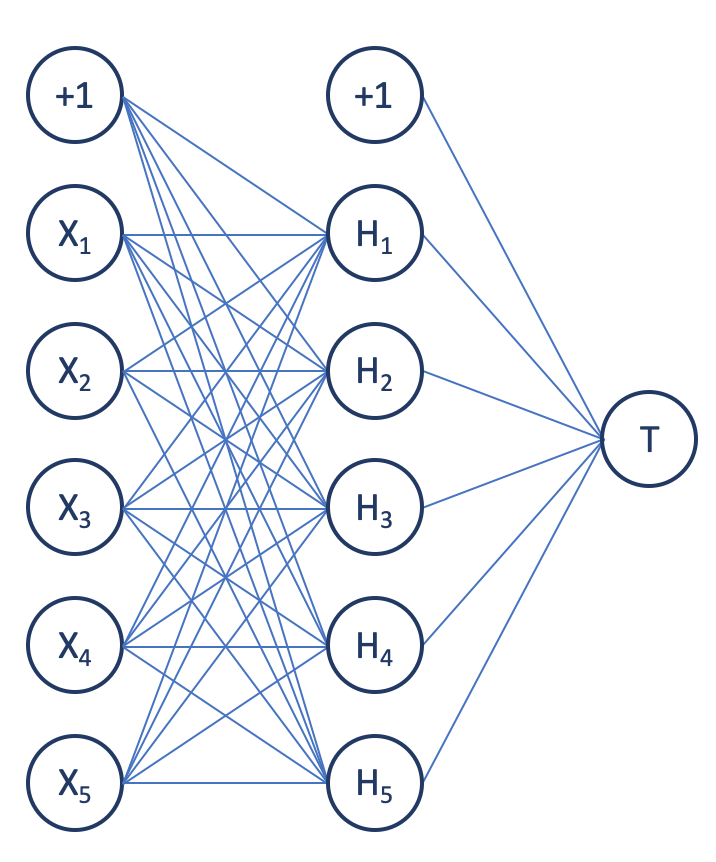
\includegraphics[width=.3\textwidth]{nnp2.png}

We use $w_{ij}$ to represent the weight between $X_i$ and $H_j$,  and use $w_{0j}$ to represent the weight between the first layer bias term (+1) and $H_j$. We use $v_i$ to represent the weight between $H_i$ and $T$, and use $v_0$ to represent the weight between the second layer bias term (+1) and $T$.

Now, let $X_i \in \{ +1, -1\}$, $H_j = sign\left(\sum^{5}_{i=0} w_{ij}X_i\right)$, and $T = sign\left(\sum^{5}_{i=0} v_{i}H_i\right)$. 

\begin{enumerate}
    \item { Specify $w_{ij}$ such that $H_j$ is $+1$ if there are at least $j$ positive values among $X_1, X_2, X_3, X_4, X_5$, otherwise $-1$. If there are multiple acceptable weights, you only need to write down one of them. \problemworth{8}
    
    \solution{}

    }
    \item { Given $w_{ij}$ and $H_j$ defined as above, specify $v_i$ such that the whole neural network behaves like the XOR operation of $X_1, X_2, X_3, X_4, X_5$. If there are multiple acceptable weights, you only need to write down one of them. \problemworth{8}
    
    \solution{}
    }
    
    \item { Justify why the output of the neural network behaves like the XOR operation of $X_1, X_2, X_3, X_4, X_5$. \problemworth{4}
    
    \solution{}
    }
\end{enumerate}

\section{Implementation: Digit Recognizer \problemworth{48}}

In this exercise, you will implement a digit recognizer in pytorch. Our data contains pairs of $28 \times 28$ images $\mathbf{x}_n$ and the corresponding digit labels $y_n \in \{0, 1, 2\}$. For simplicity, we view a $28 \times 28$ image $\mathbf{x}_n$ as a 784-dimensional vector by concatenating the row pixels. In other words, $\mathbf{x}_n \in \mathbb{R}^{784}$. Your goal is to implement two digit recognizers (\verb|OneLayerNetwork| and \verb|TwoLayerNetwork|) and compare their performances.


\rule{\textwidth}{1pt}
code and data
\begin{itemize}[nolistsep]
\item \href{https://colab.research.google.com/drive/1eBjmXxPAiJaK2FoKFDhyrG5Xc49pMPyt?usp=sharing}{code} : \verb|Fall2020-CS146-HW3.ipynb|
\item \href{https://drive.google.com/drive/folders/1UHUD_a1RtRW74H0TrC8pAoO6vDSXyns3?usp=sharing}{data} : \verb|hw3_train.csv|, \verb|hw3_valid.csv|, \verb|hw3_test.csv|
\end{itemize}
\rule{\textwidth}{1pt}

Please use your \textit{@g.ucla.edu} email id to access the code and data. Similar to \textit{HW-1}, copy the colab notebook to your drive and make the changes. Mount the drive appropriately and copy the shared data folder to your drive to access via colab. For colab usage demo, check out the Discussion recordings for Week 2 in CCLE. 
The notebook has marked blocks where you need to code. \\
\\
 $\#\#\# ========= TODO  : START ========= \#\#\#$
 
 $\#\#\# ========= TODO :  END   ========== \#\#\#$

\textbf{Note: For the questions requiring you to complete a piece of code, you are expected to {\color{red}copy-paste your code as a part of the solution} in the submission pdf. Tip: If you are using \LaTeX, check out the Minted package (\href{https://www.overleaf.com/learn/latex/Code_Highlighting_with_minted}{example}) for code highlighting.} 

\vspace{10pt} {\large \textbf{Data Visualization and Preparation}
\problemworth{10}}
\begin{enumerate}
\item Randomly select three training examples with \emph{different labels} and print out the images by using \verb|plot_img| function. Include those images in your report. \problemworth{2}

\solution{}

\item The loaded examples are numpy arrays. Convert the numpy arrays to tensors. \problemworth{3}

\solution{}

\item Prepare \verb|train_loader|, \verb|valid_loader|, and \verb|test_loader| by using \verb|TensorDataset| and \verb|DataLoader|. We expect to get a batch of pairs $(\mathbf{x}_n, y_n)$ from the dataloader. Please set the batch size to 10. \problemworth{5}

You can refer \url{https://pytorch.org/docs/stable/data.html} for more information about \verb|TensorDataset| and \verb|DataLoader|.

\solution{}
\end{enumerate}



\vspace{10pt} {\large \textbf{One-Layer Network} \problemworth{15}}

For one-layer network, we consider a \emph{784--3} network. In other words, we learn a $784 \times 3$ weight matrix $\mathbf{W}$. Given a $\mathbf{x}_n$, we can compute the probability vector $\mathbf{p}_n = \sigma(\mathbf{W}^\top \mathbf{x}_n)$, where $\sigma(.)$ is the element-wise sigmoid function and $\mathbf{p}_{n,c}$ denotes the probability of class $c$. Then, we focus on the \emph{cross entropy loss}
\[ -\sum\limits_{n=0}^{N} \sum\limits_{c=0}^{C}  \mathds{1}(c=y_n) \log (\mathbf{p}_{n, c})\]
where $N$ is the number of examples, $C$ is the number of classes, and $\mathds{1}$ is the indicator function.


\begin{enumerate}[resume]
\item Implement the constructor of \verb|OneLayerNetwork| with \verb|torch.nn.Linear| and implement the \verb|forward| function to compute the outputs of the single fully connected layer i.e. $\mathbf{W}^\top \mathbf{x}_n$. Notice that we do not compute the sigmoid function here since we will use \verb|torch.nn.CrossEntropyLoss| later. \problemworth{5}

You can refer to \url{https://pytorch.org/docs/stable/generated/torch.nn.Linear.html} for more information about \verb|torch.nn.Linear| and refer to \url{https://pytorch.org/docs/stable/generated/torch.nn.CrossEntropyLoss.html} for more information about using \verb|torch.nn.CrossEntropyLoss|.

\solution{}

\item Create an instance of \verb|OneLayerNetwork|, set up a criterion with \verb|torch.nn.CrossEntropyLoss|, and set up a SGD optimizer with learning rate 0.0005 by using \verb|torch.optim.SGD| \problemworth{2}

\solution{}

You can refer to \url{https://pytorch.org/docs/stable/optim.html} for more information about \verb|torch.optim.SGD|.

\item Implement the training process. This includes forward pass, initializing gradients to zeros, computing loss, loss backward, and updating model parameters. If you implement everything correctly, after running the \verb|train| function in main, you should get results similar to the following. \problemworth{8}

\begin{minted}{text}
Start training OneLayerNetwork...
| epoch  1 | train loss 1.075387 | train acc 0.453333 | valid loss ...
| epoch  2 | train loss 1.021301 | train acc 0.563333 | valid loss ...
| epoch  3 | train loss 0.972599 | train acc 0.630000 | valid loss ...
| epoch  4 | train loss 0.928335 | train acc 0.710000 | valid loss ...
...
\end{minted}

\solution{}

\end{enumerate}


\vspace{10pt} {\large \textbf{Two-Layer Network} \problemworth{7}}

For two-layer network, we consider a \emph{784--400--3} network. In other words, the first layer will consist of a fully connected layer with $784 \times 400$ weight matrix $\mathbf{W}_1$ and a second layer consisting of $400 \times 3$ weight matrix $\mathbf{W}_2$. Given a $\mathbf{x}_n$, we can compute the probability vector $\mathbf{p}_n = \sigma(\mathbf{W}_2^\top \sigma(\mathbf{W}_1^\top \mathbf{x}_n))$, where $\sigma(.)$ is the element-wise sigmoid function. Again, we focus on the \emph{cross entropy loss}, hence the network will impelement $\mathbf{W}_2^\top \sigma(\mathbf{W}_1^\top \mathbf{x}_n)$ (note the outer sigmoid will be taken care of implicitly in our loss).


\begin{enumerate}[resume]
\item Implement the constructor of \verb|TwoLayerNetwork| with \verb|torch.nn.Linear| and implement the \verb|forward| function to compute $\mathbf{W}_2^\top \sigma(\mathbf{W}_1^\top \mathbf{x}_n)$. \problemworth{5}

\solution{}

\item Create an instance of \verb|TwoLayerNetwork|, set up a criterion with \verb|torch.nn.CrossEntropyLoss|, and set up a SGD optimizer with learning rate 0.0005 by using \verb|torch.optim.SGD|. Then train \verb|TwoLayerNetwork|. \problemworth{2}

\solution{}

\end{enumerate}

\vspace{10pt} {\large \textbf{Performance Comparison} \problemworth{16}}

\begin{enumerate}[resume]
\item Generate a plot depicting how \verb|one_train_loss|, \verb|one_valid_loss|, \verb|two_train_loss|, \verb|two_valid_loss| varies with epochs. Include the plot in the report and describe your findings. \problemworth{3}

\solution{}

\item Generate a plot depicting how \verb|one_train_acc|, \verb|one_valid_acc|, \verb|two_train_acc|, \verb|two_valid_acc| varies with epochs. Include the plot in the report and describe your findings. \problemworth{3}

\solution{}

\item Calculate and report the test accuracy of both the one-layer network and the two-layer network. Explain why we get such results. \problemworth{3}

\solution{}

\item {Replace the SGD optimizer with the Adam optimizer and do the experiments again. Show the loss figure, the accuracy figure, and the test accuracy. Include the figures in the report and describe your findings. \problemworth{7}

You can refer to \url{https://pytorch.org/docs/stable/optim.html} for more information about \verb|torch.optim.Adam|.

\solution{}

}


\end{enumerate}



\section*{Submission instructions for programming problems}
\begin{itemize}
\item Please export the notebook to a $\verb|.py|$ file by clicking the “File” $\rightarrow$ “Download.py” and upload to CCLE. 

Your code should be commented appropriately. The most important things:
\vspace{-\parskip}
\begin{itemize}[nosep]
\item Your name and the assignment number should be at the top of each file.
\item Each class and method should have an appropriate doctsring.
\item If anything is complicated, it should include some comments.
\end{itemize}
\vspace{-\parskip}
There are many possible ways to approach the programming portion of this assignment, which makes code style and comments very important so that staff can understand what you did. For this reason, you will lose points for poorly commented or poorly organized code.
\end{itemize}

\begin{itemize}
\item Please submit all the plots and the rest of the solutions (other than codes) to Gradescope
\end{itemize}


\end{document}